\documentclass[../../../../../../../dd.tex]{subfiles}

\begin{document}

	\subsubsection{IO Manager}
		This component will be implemented using the Command Pattern (see \href{https://it.wikipedia.org/wiki/Command_pattern}{Command Pattern on Wikipedia}).
		It will contain the following main classes, in general for each functionality of the UI there is a Message class that, for the sake of brevity, are not all listed:
		\begin{itemize}
			\item \textbf{Message Type} (Interface) \textbf{:} this sub-component is the Interface which is extended by each Message class. 

			\item \textbf{Message Types:} this sub-component is an enumeration in which each enumeration entry returns an implementation of the Message Type Interface.

			\item \textbf{Message Types Map:} this sub-component is an Hash Map that associates the name of the elements of the enumeration, the enumeration element identified by that name.

			\item \textbf{Messages Handler:} this sub-component receives messages from the View classes. It selects the right message to send by processing the message name and selecting (through the Message Type Map) the right Message Class.

			\item \textbf{Request Message:} This sub-component is in charge to call Requests and Reservations functions to add a Taxi Request in the myTaxiService database.

			\item \textbf{Reservation Message:} This sub-component is in charge to call Requests and Reservations functions to add a Taxi Reservation in the myTaxiService database.

			\item \textbf{Customer Notification Message:} This sub-component is used to send notifications to a Customer. These notifications are used mainly to confirm to a Customer that his request has been handled.

			\item \textbf{TaxiDriver Notification Message:} This sub-component is used to send notifications to a Taxi Driver. These notifications are mainly used to advise a Taxi Driver that he's been selected for a certain ride request.

			\item \textbf{Login Message:} This sub-component is in charge to forward login requests from users to the Profile Manager.

			\item \textbf{Registration Message:} This sub-component is in charge to forward registration requests from users to the Profile Manager.

			\item \textbf{Ok Message:} This sub-component is used to send success notifications to a specific user.

			\item \textbf{Error Message:} This sub-component is used to send error notifications to a specific user.

			\item \textbf{End Ride Message:} This sub-component is in charge to call the functions of the Requests and Reservations Manager that can set as ended a ride. An End Ride Message is sent by the client applications to signal that a ride is ended.

			\item \textbf{Profile Modification Message:} This sub-component is in charge to call the functions of the Profile Manager that can modify a user profile.
			
		\end{itemize}

		\begin{figure}[H]
				\centering
				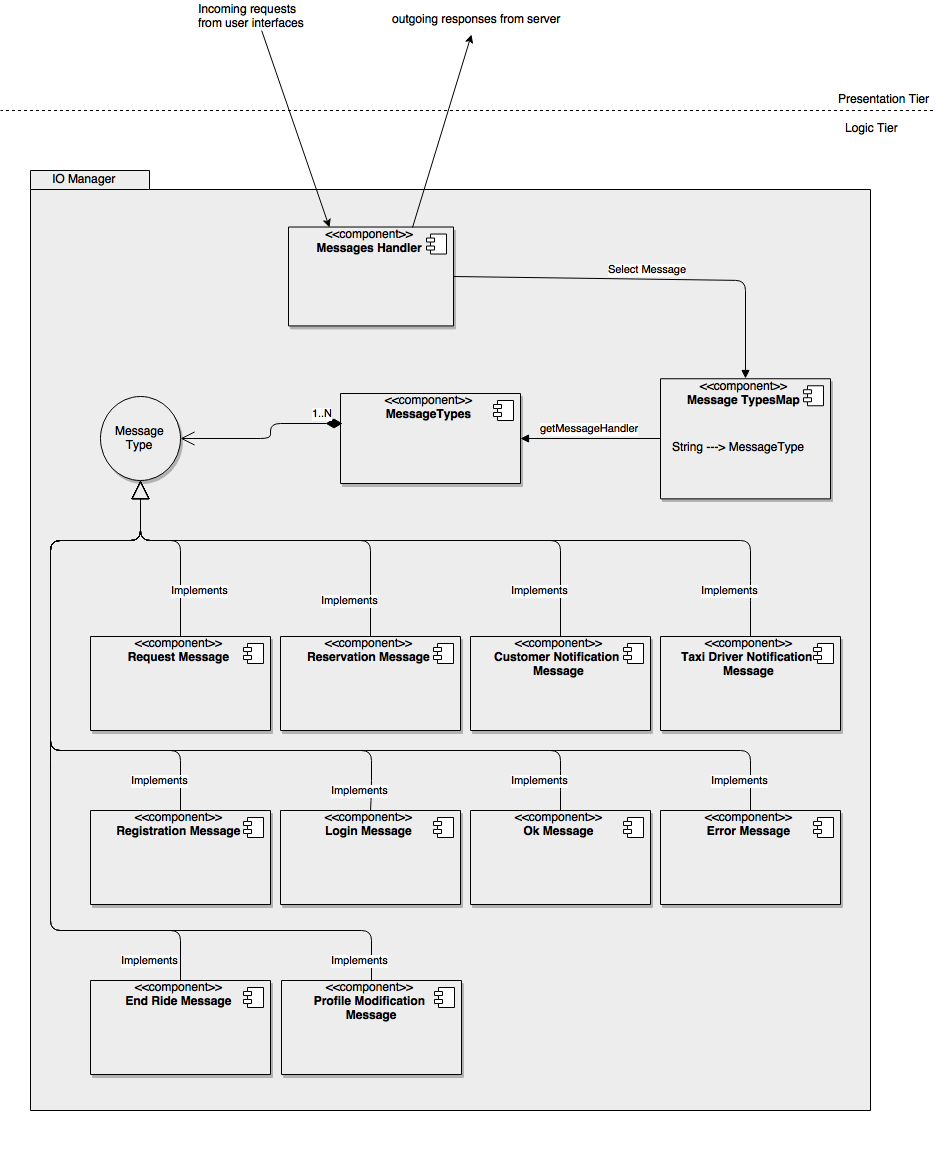
\includegraphics[width=\textwidth, scale=0.5]{../images/IOManager.png}
			\caption{IO Manager Structure}\label{fig:IOManager}
		\end{figure}
	
\end{document}